\subsection{Remote Video Streaming}
\label{subsec:remote-video-streaming}

Wie in Kapitel \ref{subsubsec:video-streaming} gezeigt, kann der \gls{go1} die Bilder der fünf verbauten Kameras über
ein Netzwerk streamen.
Dieses Kapitel baut auf den Erkenntnissen des Kapitels \ref{subsubsec:video-streaming} auf und erweitert die dort gezeigten
Funktionen um den Streaming-Server und eine Darstellung des gestreamten Kamerabildes.

\myparagraph{Vorbereitung}

Zur Vorbereitung des Remote Videostreaming muss zuerst ein Streaming-Server vorbereitet werden, der über eines der am
Roboter verbundenen Netzwerke erreichbar ist.
In diesem Kapitel wird zum einfachen Hosting des Servers die Virtualisierungsumgebung \emph{Docker} verwendet.
Ein vorhandenes Grundwissen hierüber wird vorausgesetzt, jedoch ist die Anwendung sehr einfach gehalten.
Docker hat hier den Vorteil, dass das gezeigte Beispiel auf den meisten Rechnern nachstellbar ist.
Der eigentlich verwendete Server ist somit nicht relevant, insofern Docker auf ihm installiert werden kann.

Die Open-Source-Bibliothekssammlung \emph{bluenvironment} enthält eine auf der Programmiersprache \emph{GO} besierte
Implementierung eines Medienservers mit Unterstützung diverser Videoprotokolle wie beispielsweise \gls{rtsp} und
\gls{webrtc}.
Diese werden auch im folgenden Beispiel verwendet.
Die Implementierung des Medienservers ist zur Nutzung als Docker-Image verfügbar, welches über folgenden Befehl
genutzt werden kann.

\begin{lstlisting}[language=Bash]
docker run --rm -it \
    -e MTX_PROTOCOLS=tcp \
    -p 8554:8554 \
    -p 8889:8889 \
\end{lstlisting}

Führt man diesen Befehl auf dem zu nutzenden externen Server aus, so startet das Image einen Container mit integriertem
Medienserver, welcher für das Streaming über das Protokoll \gls{rtsp} den Port \num{8554} und für das Protokoll \gls{webrtc}
den Port \num{8889} öffnet und auf dem Host verfügbar macht.
Für das Empfangen der Kamera-Streams des \gls{go1} wird in diesem Fall \gls{rtsp} verwendet, für das Senden eines Streams
hingegen \gls{webrtc}.
Sobald der Container gestartet ist, wartet der Medienserver auf Verbindungen.

\myparagraph{Streaming}

Das Streaming der Kamerabilder vom Roboter auf den Server verläuft analog zu der Vorgehensweise in Kapitel \ref{subsubsec:video-streaming}.

\begin{lstlisting}[language=Bash]
ffmpeg -nostdin \                  # Keine Interaktion
    -f video4linux2 \              # Input Format
    -i /dev/video1 \               # Input-URL
    -vcodec libx264 \              # Video Kodierung (h264)
    -preset:v ultrafast \          # Kodierungsgeschwindigkeit
    -tune zerolatency \            # Keine H264 B-Frames
    -framerate 5 \                 # Framerate
    -f rtsp \                      # Output Format
    rtsp://<ip:8554|port>/<stream> # Output File/URL
\end{lstlisting}

Hier ist nun die Server \gls{ip} aus dem vorigen Paragrafen in der letzten Zeile des Befehls einzusetzen, gefolgt vom Port
\num{8554} für das \gls{rtsp}.
Als Stream Name kann ein selbst gewählter Begriff genutzt werden.
Streamt man mehrere Kameras gleichzeitig, so bietet es sich an, die Namen nach Ausrichtung der Kamera zu benennen.
Für den Stream der nach vorne gerichteten Kameras des \gls{go1} bietet sich beispielsweise folgende Server-\gls{url} an:

\begin{lstlisting}[language=Bash]
rtsp://192.168.123.70:8554/head
\end{lstlisting}

\noindent Nach erfolgreicher Verbindung wird auf dem Server folgende Meldung ausgegeben.

\begin{lstlisting}[language=Bash]
2023/08/25 10:22:02 INF [RTSP] [conn 192.168.123.13:35428] opened
2023/08/25 10:22:02 INF [RTSP] [session f35fae28] created by 192.168.123.13:35428
2023/08/25 10:22:02 INF [RTSP] [session f35fae28] is publishing to path 'head', with TCP, 1 track (H264)
\end{lstlisting}

\noindent Auf dem Nano im Kopf des Roboters wird folgende Meldung ausgegeben.

\begin{lstlisting}[language=Bash]
Output #0, rtsp, to 'rtsp://192.168.123.52:8554/head':
  Metadata:
    encoder         : Lavf57.83.100
    Stream #0:0: Video: h264 (libx264), yuvj422p(pc), 928x400, q=-1--1, 100 fps, 90k tbn, 100 tbc
    Metadata:
      encoder         : Lavc57.107.100 libx264
    Side data:
      cpb: bitrate max/min/avg: 0/0/0 buffer size: 0 vbv_delay: -1
frame=15476 fps=101 q=24.0 size=N/A time=00:02:34.75 bitrate=N/A dup=11652 drop=0 speed=1.01x
\end{lstlisting}

\noindent Die Kamerabilder des Kopfes werden erfolgreich übertragen.
Diese Vorgehensweise kann für alle anderen Kameras wiederholt werden, es muss lediglich ein neuer Stream unter einem anderen
Namen an den Server gesendet werden.

\myparagraph{Anzeigen des Streams}

Das Protokoll \gls{webrtc} hat den Vorteil, dass es in den meisten modernen Browsern bereits unterstützt wird und
keinerlei Konfiguration bedarf.
Zum Anzeigen der Kamerabilder kann einfach die Server \gls{url} inklusive des Ports und des Stream-Namens in die
Adressleiste des Browsers eingegeben werden.
Das Kamerabild im Browser wird wie in Abbildung \ref{fig:browser} gezeigt dargestellt.

\begin{figure}[h]
    \frame{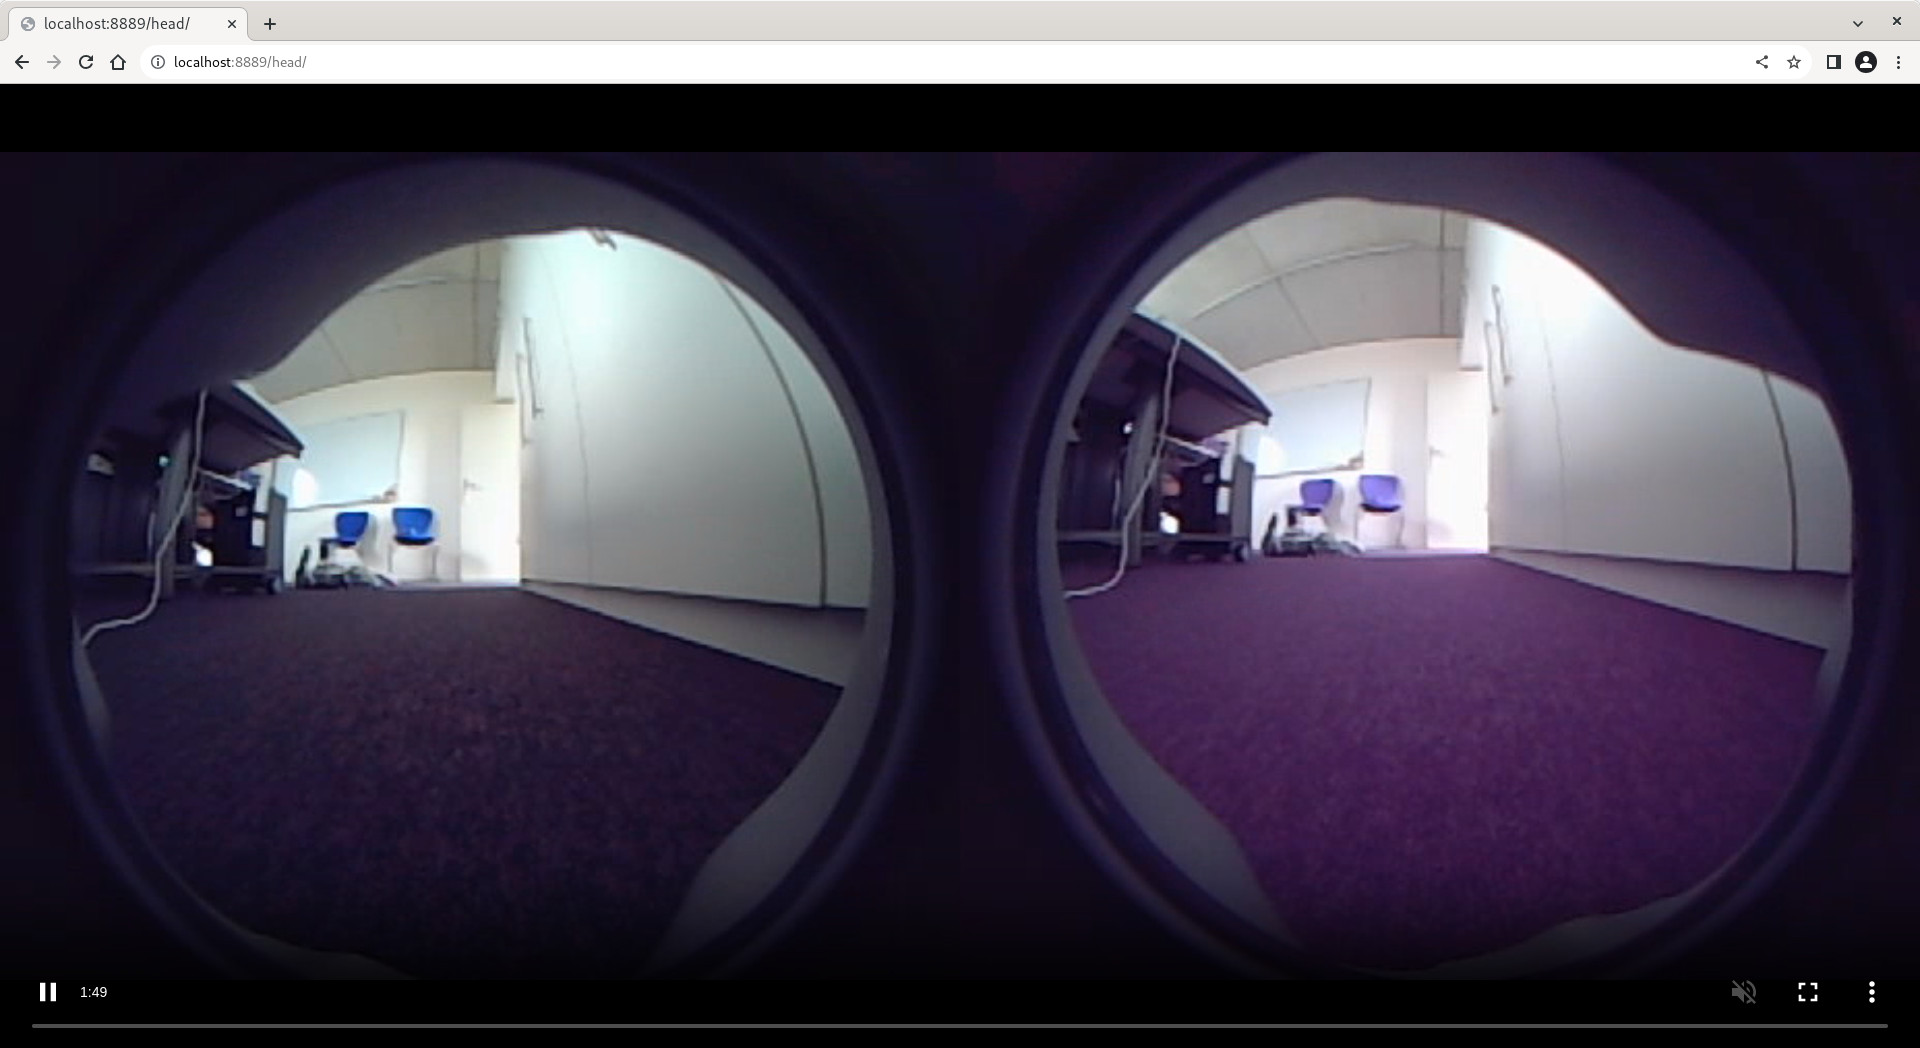
\includegraphics[width=\linewidth]{img/erweiterung/browser-webrtc}}
    \caption{Das Kamerabild des Kopfes in der Browseransicht}\label{fig:browser}
\end{figure}

Getestet wurde für dieses Beispiel auf dem Browser \emph{Chromium} in der Version
\texttt{116.0.5845.96 (Official Build) built on Debian 12.1, running on Debian 12.1 (64-bit)}.


